\begin{figure}
    \begin{subfigure}{.5\textwidth}
        \centering
        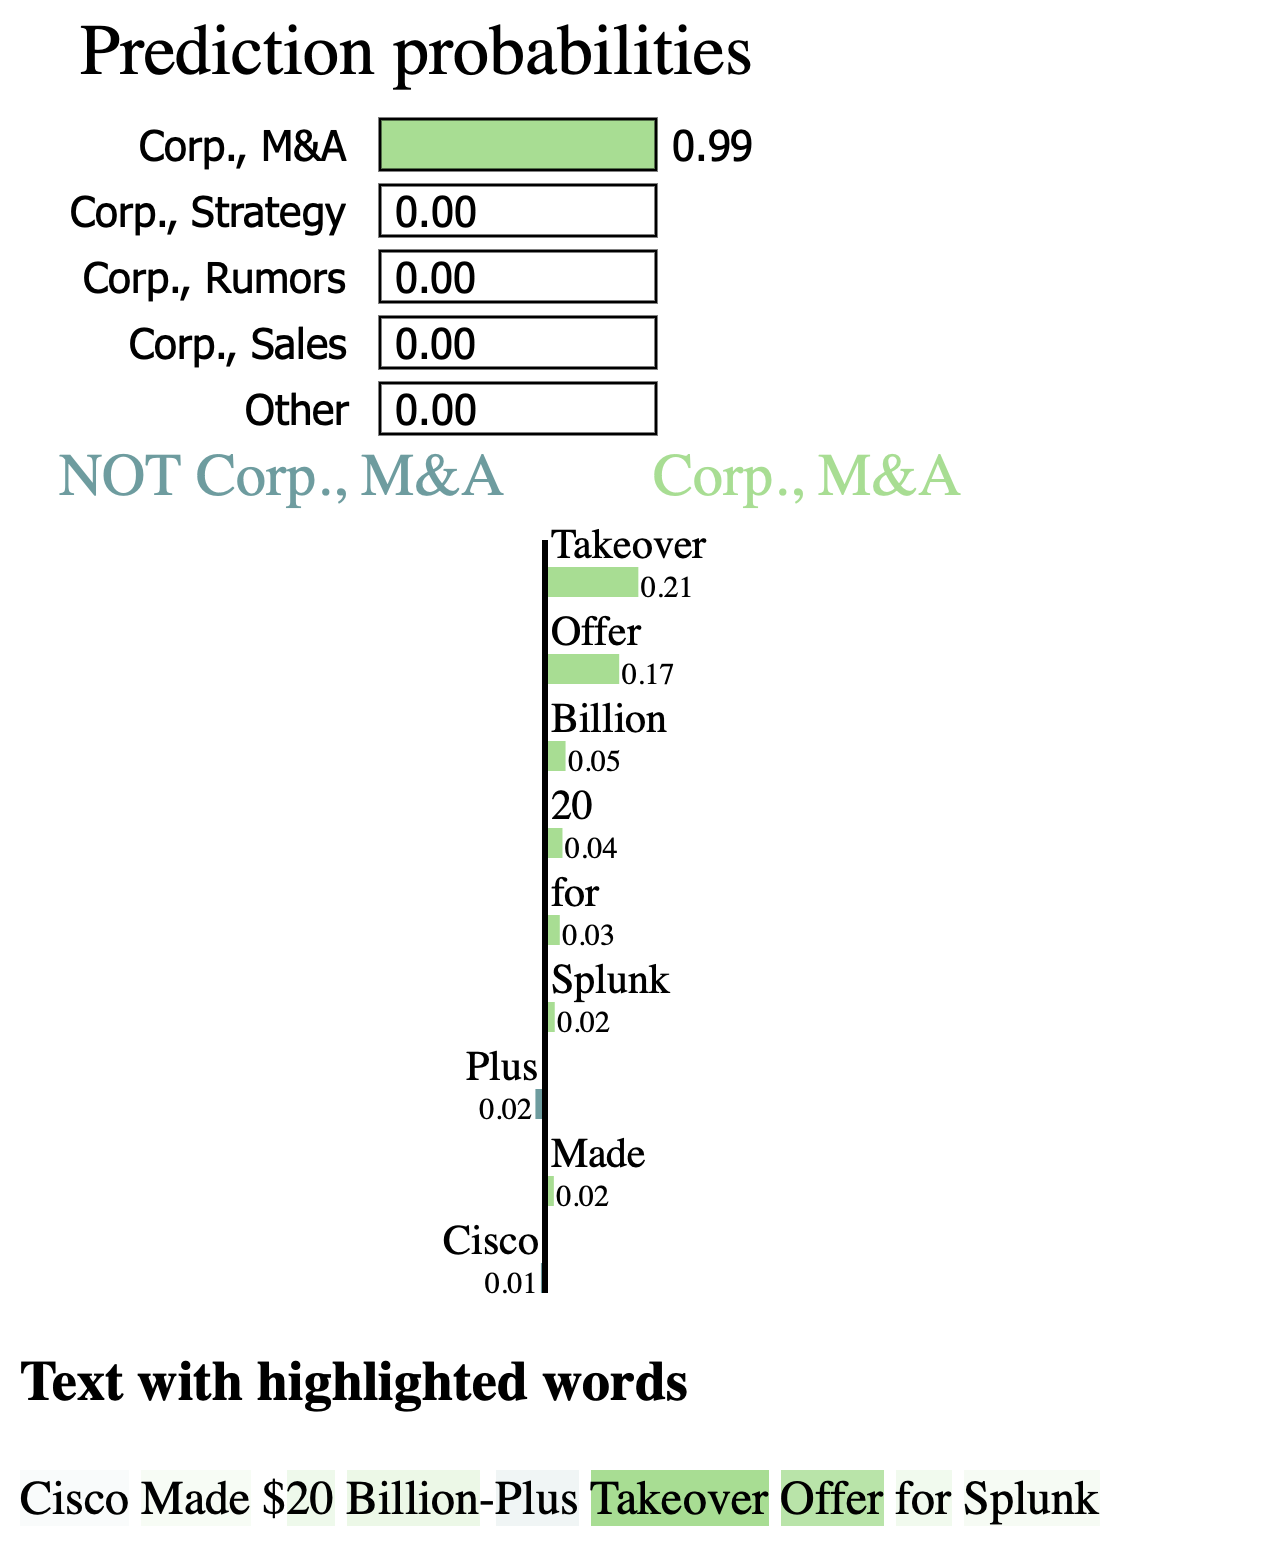
\includegraphics[width=.8\linewidth]{images/lime_m&a.png}
        \label{fig:lime1}
    \end{subfigure}%
    \begin{subfigure}{.5\textwidth}
        \centering
        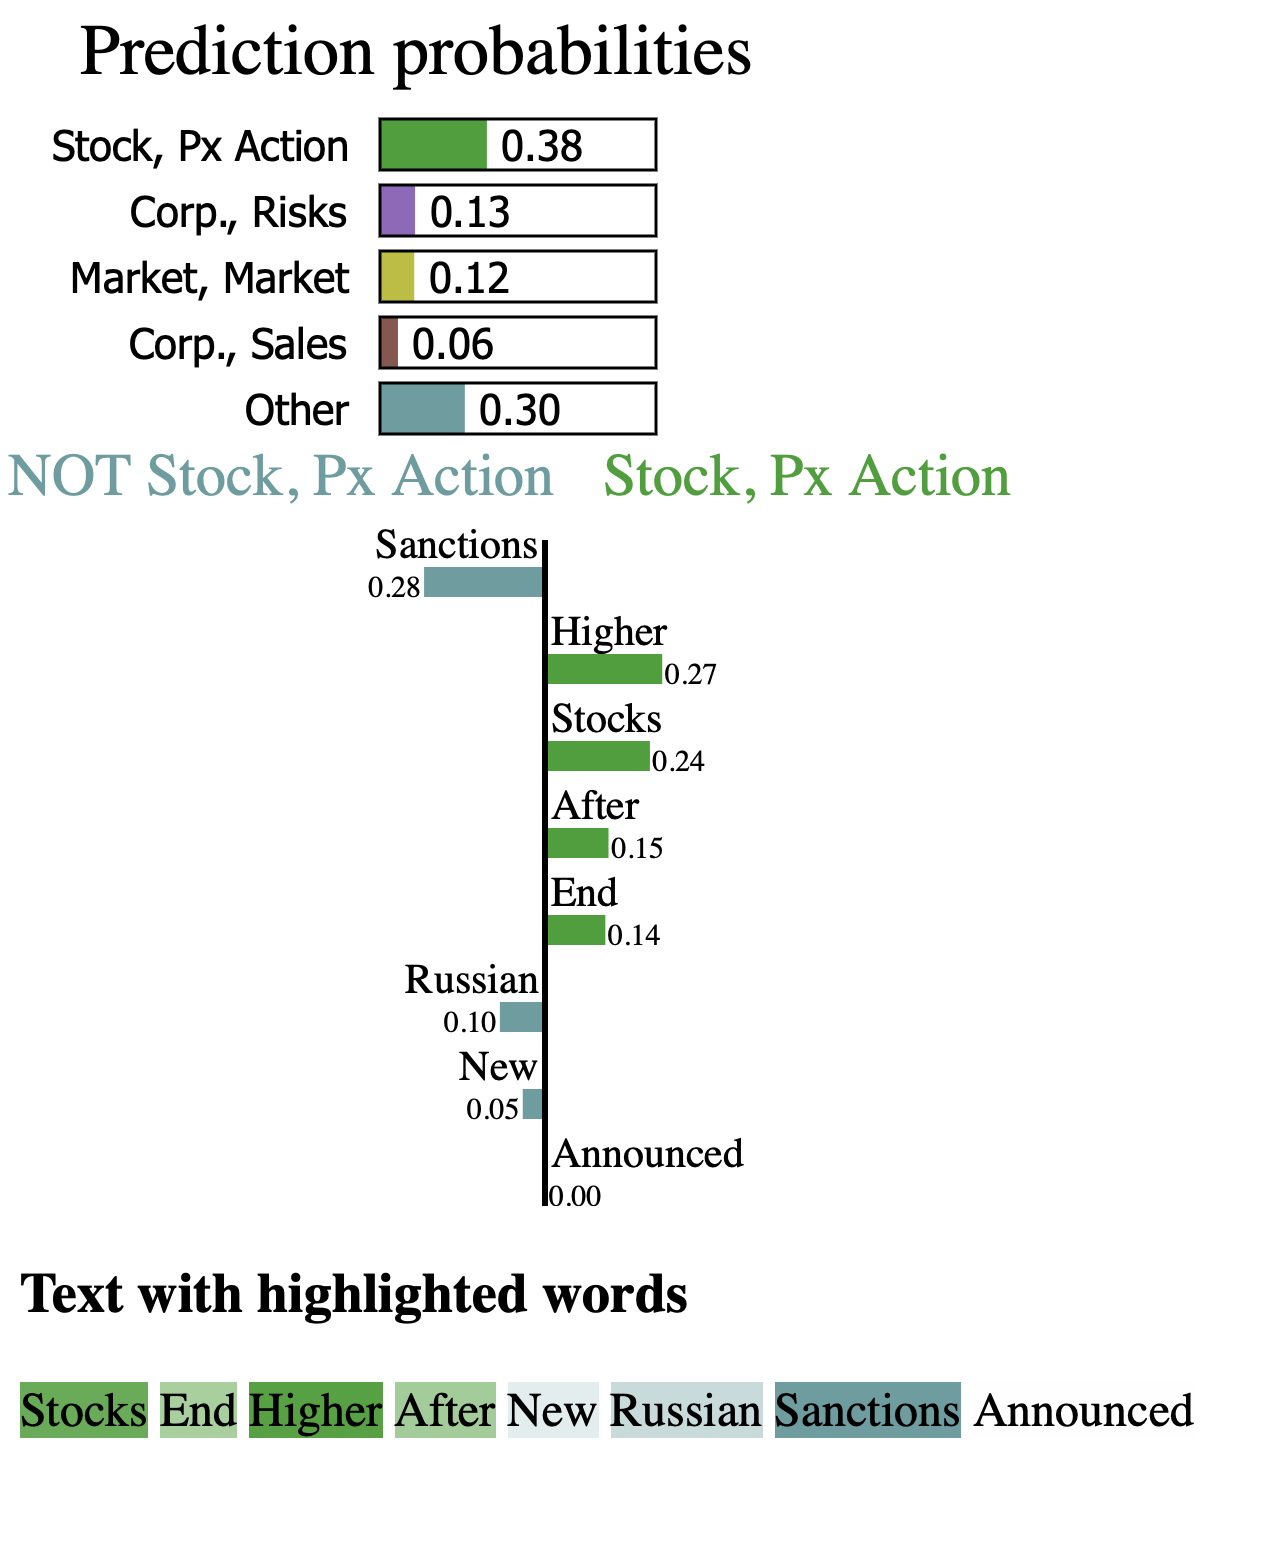
\includegraphics[width=.8\linewidth]{images/lime_price_action_2.png}
        \label{fig:lime3}
    \end{subfigure}
    \caption{LIME Plots of Out-Of-Sample Financial Headlines}
    \label{fig:fig}
\end{figure}

To aid the interpretability of our model, we train multiple locally interpretable model-agnostic explanations (LIME) models~\citep{lime2016} on recent out-of-sample headlines from the Wall Street Journal.

LIME works by perturbing the input sentence, deleting random words.
Using our neural baseline model, LIME then makes aspect class predictions on the perturbed sentence.
These predictions are used to fit a linear regression model.
The resulting LIME model shows the contribution of each word to the neural baseline’s prediction.

Looking at the LIME visuals in figure~\ref{fig:fig}, sometimes a keyword or two can distinguish among aspect classes.
The headline `Cisco Made \$20 Billion-Plus Takeover Offer for Splunk,' shows that the BERT model has learned to associate the phrase `Takeover Offer' with the correct class, `Corporate - M\&A.'
In another example, the phrase `Stocks end higher after' is associated with price movement.
